\chap{Sesuatu Tidak Selalu Kelihatan Sebagaimana Adanya}

\small
Dua orang malaikat berkunjung ke rumah sebuah keluarga kaya. Keluarga itu sangat kasar dan tidak mengijinkan kedua malaikat itu bermalam di ruang tamu yang ada di rumahnya, malaikat tersebut ditempatkan pada sebuah kamar berukuran kecil yang ada di basement. Ketika malaikat itu hendak tidur, malaikat yang lebih tua melihat bahwa dinding basement itu retak. Kemudian malaikat itu memperbaikinya sehingga retak pada dinding basement itu lenyap dan ketika malaikat yang lebih muda bertanya mengapa ia melakukan hal itu, malaikat yang lebih tua menjawab, “sesuatu tidak selalu kelihatan sebagaimana adanya''.

Malam berikutnya, kedua malaikat itu beristirahat di rumah seorang petani dan istrinya yang miskin tetapi sangat ramah. Setelah membagi sedikit makanan yang ia punyai, petani itu mempersilahkan kedua malaikat untuk tidur di atas tempat tidurnya.

\begin{wrapfigure}{r}{1.5cm}
\centering
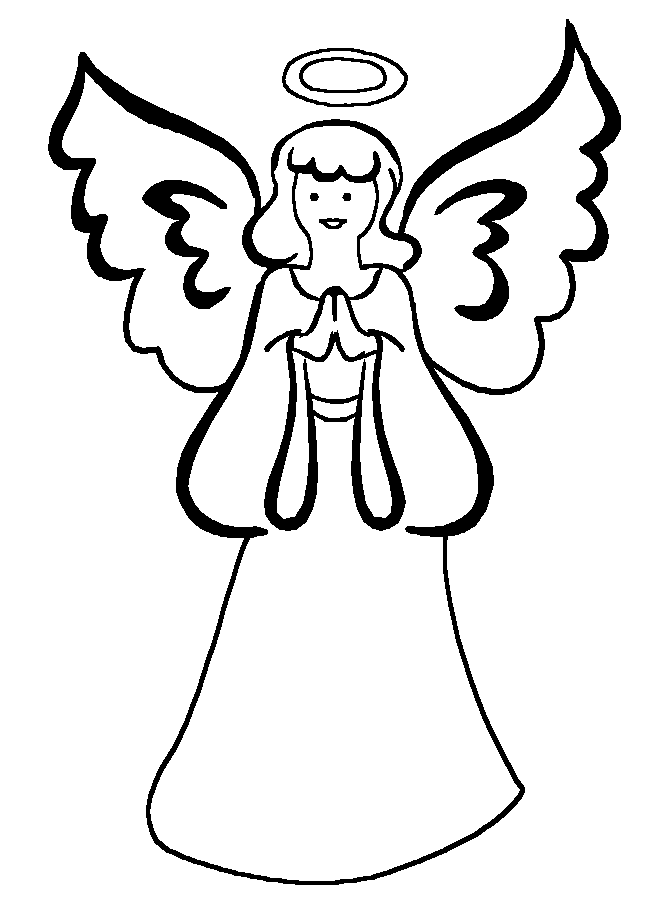
\includegraphics[scale=0.07]{gambar/malaikat.png}
\end{wrapfigure}

Ketika matahari terbit keesokan harinnya, malaikat menemukan bahwa petani itu dan istrinya sedang menangis sedih karena sapi mereka yang merupakan sumber pendapatan satu-satunya bagi mereka, terbaring mati. Malaikat yang muda merasa geram. Ia bertanya kepada malaikat yang lebih tua.
``mengapa kau membiarkan hal ini terjadi? Keluarga yang pertama memiliki segalanya, tapi engkau menolong menambalkan dindingnya yang retak. Keluarga ini hanya memliki sedikit, tetapi walaupun demikian mereka bersedia membaginya dengan kita. Mengapa engkau membiarkan sapinya mati?''

Malaikat yang lebih tua menjawab, ``sesuatu tidak selalu kelihatan sebaaimana adanya''.
``ketika kita bermalam di basement, aku melihat ada emas tersimpan di lubang dalam dinding itu. Karena pemilik rumah sangat tamak dan tidak bersedia membagi hartanya, aku menutup dinding itu agar ia tidak menemukan emas itu''.

 ``Tadi malam ketika kita tidur di ranjang petani ini, malaikat maut datang untuk mengambil nyawa istrinya, aku memberikan sapinya agar malaikat maut tidak jadi mengambil istrinya.''

\begin{wrapfigure}{l}{1cm}
\centering

\includegraphics[scale=0.09]{gambar/malaikat2.png}
\end{wrapfigure}

MEMANG, ``Terkadang Sesuatu Tidaklah Tampak Sebagaimana Kelihatannya''. Kadang-kadang itulah yang kita rasakan ketika berpikir bahwa sesuatu tidaklah seharusnya terjadi.

Jika kita punya iman, kita hanya perlu percaya bahwasanya semua hal yang terjadi adalah demi kebaikan kita. Kita tidak menyadari hal itu sampai saatnya tiba.

\sumber{``Sesuatu Tidak Selalu Kelihatan Sebagaimana Adanya.''\\
 www.renungan-harian-kita.blogspot.com.}
\normalsize